\chapter{Theoretical background}
\label{chap2} % id kapitoly pre prikaz ref

\section*{Implicit surfaces}
\label{sub2.1}

Implicit functions are a tool for surface representation and manipulation.
In computer graphics, they can be used for modelling of complex surfaces
using boolean operations, realistic animations, rendering and other.

Implicit functions do not define the boundary explicitly, instead
the surface is defined as a zero set of a function.
\begin{definition}
    Given a function $F: \R^3 \to \R$, one can define an implicit surface
    as a set of points that fullfil $F(x, y, z) = 0$.
\end{definition}

Some examples of implicit surfaces and their equations can be seen on
image \ref{img:1}.

\begin{figure}
    \centerline{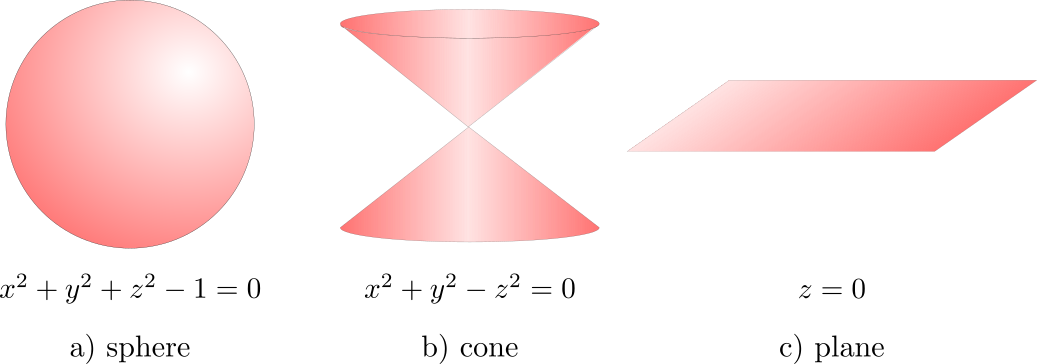
\includegraphics[width=0.85\textwidth]{images/img1}}
    \caption[Implicit surfaces with corresponding equations]
    {Implicit surfaces with corresponding equations.}
    %id obrazku, pomocou ktoreho sa budeme na obrazok odvolavat
    \label{img:1}
\end{figure}

Normal vector of the implicit surface in point $(x_0, y_0, z_0)$ is
normalized gradient of the implicit function in that point.

\begin{definition}
    Gradient vector of an implicit function $F:\R^3 \to \R$ is defined as 
    $$\nabla F(x, y, z) = \bigg(\frac{\partial F(x, y, z)}{\partial x}, \frac{\partial F(x, y, z)}{\partial y}, 
    \frac{\partial F(x, y, z)}{\partial z}\bigg).$$
    If $\nabla F(x,y,z) \neq 0$, we can define normal vector of $F$ as 
    a normalized gradient vector
    $$N(F(x, y, z))  = \frac{\nabla F(x, y, z)}{\| \nabla F(x, y, z) \|} \,\,\,\,\,\, for \,\,\,\,\,\,
    \nabla F(x,y,z) \neq 0.$$
    \\*
\end{definition}

Points lying on the implcit surface can be classified as regular or
singular based on the value of the gradient vector in that point.

\begin{definition}
    Point $P=(x,y,z)$ lying on the implicit surface is said to be regular,
    if $\nabla F(x, y, z) \neq 0$. On the contrary, point $P$ is said to be 
    singular, if $\nabla F(x, y, z) = 0$.
\end{definition}

Singular points can be further classified as isolated or non-isolated
based on their surroundings.

\begin{definition}
    Singular point $P$ is said to be isolated, if there exists an open ball
    $B_\varepsilon(P)$, which does not contain any other singular point.
    Singular point P is said to be non-isolated if it is not isolated.
\end{definition}

On the image \ref{img:2} we can see example of isolated and non-isolated
singularities.

\begin{figure}
    \centerline{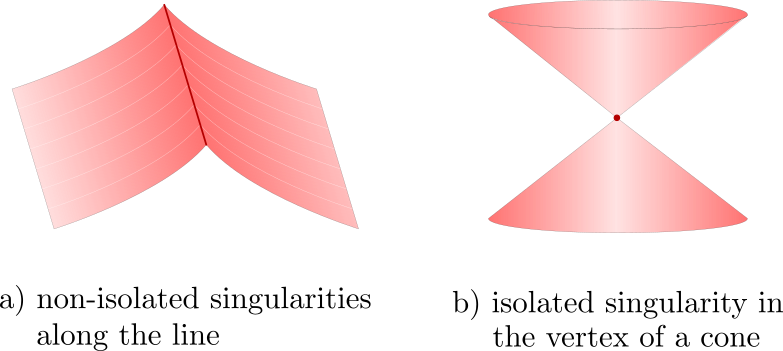
\includegraphics[width=0.6\textwidth]{images/img2}}
    \caption[Isolated and non-isolated singularity]
    {Isolated and non-isolated singularity.}
    %id obrazku, pomocou ktoreho sa budeme na obrazok odvolavat
    \label{img:2}
\end{figure}

\section*{ADE singularities}
\label{sub2.2}

ADE singularities, also reffered to as du Val singularities are a specific
class of simple, isolated surface singularities. They were first TODO.

\subsection*{ADE classification and simply laced Dynkin diagrams}
\label{subs2.2.1}

\begin{definition} \cite{humphreys2012introduction}
    A vector space $L$ over field $F$, with an operation $L \times L \to L$,
    denoted $(x, y) = [xy]$ and called the bracket or commutator of x and y,
    is called Lie algebra over $F$ if the following axioms are satisfied:
    \begin{itemize}
        \item The bracket operation is bilinear.
        \item $[xx] = 0$ for all $x$ in $L$.
        \item $[x[yz]]+[y[zx]]+[z[xy]] = 0$ for all $x, y, z \in L$.
    \end{itemize}

    Simple Lie algebra is non-abelian Lie algebra, which contains no
    nonzero proper ideals.

    Semisimple Lie algebra is a direct sum of simple Lie algebras.
\end{definition}

There is a one-to-one Correspondence between Lie algebras and Lie groups.

Dynkin diagrams are graphs which classify semisimple Lie algebras (or
equivalently semisimple Lie groups).
Simply laced Dynkin diagrams are undirected diagrams with
no multiple edges. Lie algebras which correspond to simply laced
Dynkin diagrams are called simply laced Lie algebras.

ADE in ADE singularities reffers to ADE classification, which is used when
some objects have a pattern that corresponds to simply laced Dynkin diagrams.

Simple Lie algebras over algebraically closed field 
(and their corresponding Lie groups) are
classified based on their Dynkin diagrams as
\begin{itemize}
\item $A_n$ \hspace{3mm}  $n>=1$,
\item $B_n$ \hspace{3mm}  $n>=2$,
\item $C_n$ \hspace{3mm}  $n>=3$,
\item $D_n$ \hspace{3mm}  $n>=4$,
\item $E_6, E_7, E_8, F_4, G_2$.
\end{itemize}
The corresponding Dynkin diagrams can be seen on image \ref{img:3}.

\begin{figure}
    \centerline{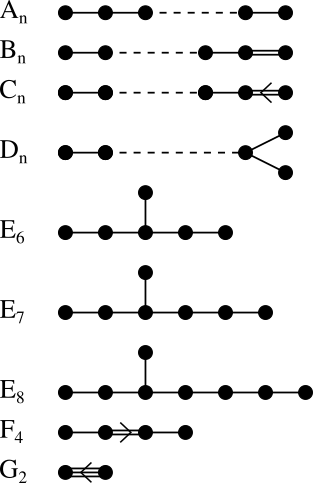
\includegraphics[width=0.3\textwidth]{images/img3}}
    \caption[Finite Dynkin diagrams]
    {Finite Dynkin diagrams\cite{wikidynkindiagram}.}
    %id obrazku, pomocou ktoreho sa budeme na obrazok odvolavat
    \label{img:3}
\end{figure}

Simply laced Dynkin diagrams are simple Dynkin diagrams with no directed
and no multiple edges. $A_n, D_n, E_6, E_7$ and $E_8$ are therefore all
simply laced Dynkin diagrams.

ADE singularities are in correspondence with simply laced Dynkin
diagrams, each ADE singularity has its corresponding simply laced Dynkin
diagram and equivalently, each simply laced Dynkin diagram corresponds
to an ADE singularity. These singularities are denoted based on their
corresponding Dynkin diagram.

The ADE surface singualrities were classified by Arnold's
\cite{arnol1972normal} and they are specified by their normal forms.
When working in complex space, each singularity has a single normal form:
\begin{itemize}
    \item $A_n$ \hspace{5mm} $F(x,y,z)=z^{n+1}+x^2+y^2$,
    \item $D_n$ \hspace{5mm} $F(x,y,z)=yx^2+y^{n-1}+z^2$,
    \item $E_6$ \hspace{5mm} $F(x,y,z)=x^3+y^4+z^2$,
    \item $E_7$ \hspace{5mm} $F(x,y,z)=x^3+xy^3+z^2$,
    \item $E_8$ \hspace{5mm} $F(x,y,z)=x^3+y^5+z^2$.
\end{itemize}

Each ADE singularity on a surface can be locally expressed by their
normal form.

In the real case, changing the signs in these equations produces different
surfaces and therefore, ADE singualrities can be further classified by their
signature.

\begin{definition}
    Let's mark real surface singularities based on their signature as follows:
    \begin{itemize}
        \item $A_{n\pm\pm}$ \hspace{5mm} $F(x,y,z)=z^{n+1}\pm x^2\pm y^2$,
              
        \item $D_{n\pm\pm}$ \hspace{5mm} $F(x,y,z)=yx^2\pm y^{n-1}\pm z^2$,
        
        \item $E_{6\pm\pm}$ \hspace{5mm} $F(x,y,z)=x^3\pm y^4\pm z^2$,
        
        \item $E_{7\pm\pm}$ \hspace{5mm} $F(x,y,z)=x^3\pm xy^3\pm z^2$,
        
        \item $E_{8\pm\pm}$ \hspace{5mm} $F(x,y,z)=x^3\pm y^5\pm z^2$.
        \end{itemize}
\end{definition}

The most common example of a surface with ADE singularity is an ordinary cone.
Given as the zero set of the function $F(x, y, z)=z^2-x^2-y^2$, cone has
a singular point $P=(0, 0, 0)$. This singular point is an example of $A_{1--}$
singularity.

\subsection*{Correspondence between $SL(2,\mathbb{C})$ group and ADE singularities}
\label{subs2.2.2}
$SL(2, \mathbb{C})$ is special linear group of degree two over complex numbers.
\begin{definition}
    $SL(2, \mathbb{C})$ is a group of unimodular (determinant is 1) matrices
    of complex numbers.

    $$SL(2, \mathbb{C}) = \bigg\{
        \begin{pmatrix}
            a & b\\ 
            c & d
          \end{pmatrix} \bigg| \hspace{1mm} a,b,c,d \in \mathbb{C}, ad-bc=1
          \bigg\}.$$
\end{definition}

Simply laced Dynkin diagrams correspond to all finite subgroups of
$S0(3,\R)$. Finite subgroups of
$SO(3,\R)$ are the rotational symmetry groups of
\begin{itemize}
    \item pyramid with $n$ vertices (cyclic subgroup $\overline{C}_n$),
    \item double pyramid with $n$ vertices (dihedral subgroup $\overline{D}_n$),
    \item platonic solids
    \begin{itemize}
        \item tetrahedron (tetrahedral subgroup $\overline{T}$)
        \item octagedron (octahedral subgroup $\overline{O}$)
        \item icosahedron (icosahedral subgroup $\overline{I}$)
    \end{itemize}
\end{itemize}

These correspond to simply laced Dynkin diagrams:
\begin{itemize}
    \item $A_n \iff \overline{C}_{n+1}$,
    \item $D_n \iff \overline{D}_{n+2}$,
    \item $E_6 \iff \overline{T}$,
    \item $E_7 \iff \overline{O}$,
    \item $E_8 \iff \overline{I}$.
\end{itemize}

The conclusion is that ADE singularities correspond to finite subgroups of
$SO(3, \R)$, which represent certain types of symmetries in $\R^3$.

\section{Non-isolated translation surface singularities}
\label{sub2.3}

\section{Non-isolated translation surface singularities}
\label{sub2.4}

\section{Tringulation of regular implicit srufaces}
\label{sub2.5}

\section{Data structures for triangulation algorithm}
\label{sub2.6}
